\section{Internal Parallelization in FPGA}
\label{clicknp:sec:optimization}

Fully utilizing the internal parallelism of FPGA is crucial for performance.
\name thoroughly exploits the parallelism within and between elements in FPGA.

\subsection{Inter-element Parallelization}
The modular architecture of \name makes it natural to exploit parallelism between different elements.
The \name toolchain maps each element to a hardware module in the FPGA.
These hardware modules are interconnected through FIFO buffers and can work in complete parallel.
Therefore, each element in a \name configuration can be viewed as a tiny independent core with custom logic.
Packets flow from one element to another along the \textit{processing pipeline}.
This type of parallelism is referred to as \textit{pipeline parallelism}.
Furthermore, if a single processing pipeline does not have enough processing power, multiple such pipelines can be replicated in the FPGA, and the data can be divided into these pipelines using load balancing elements, thereby utilizing \textit{data parallelism}.
For network traffic, there is data parallelism (at the packet level or flow level) and pipeline parallelism, which can be used to accelerate processing.
\name is very flexible and can easily configure both types of parallelism, as shown in Figure \ref{clicknp:fig:element-para}.

\begin{figure}
\centering
\begin{tabular}{c}
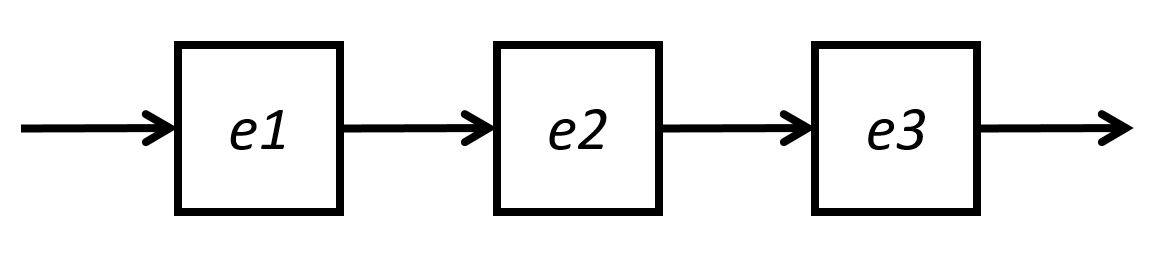
\includegraphics[width=0.56\textwidth]{pipeline.jpg}\\
(a)\\
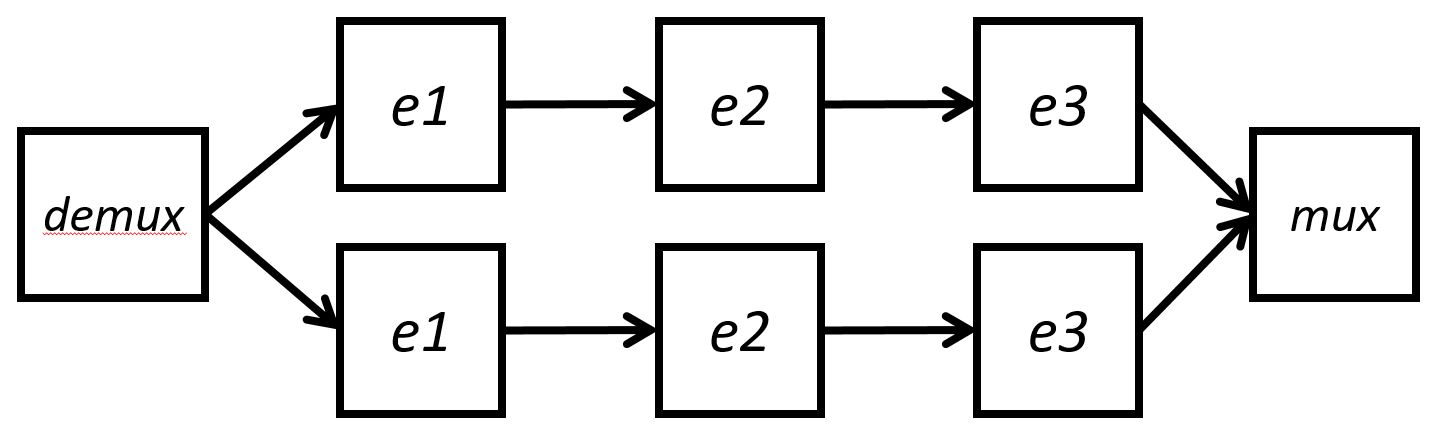
\includegraphics[width=0.7\textwidth]{data.jpg}\\
(b)\\
\end{tabular}
\caption{(a) Inter-element parallelism. (b) Intra-element parallelism.}
\label{clicknp:fig:element-para}
\end{figure}

Developers can manually specify the number of times inter-element parallelism occurs (i.e., the number of times a certain element is repeated), or they can specify the throughput or area target of the entire network function pipeline or a certain element, and the \name toolchain will automatically calculate the number of times each element is parallelized. \name obtains the average amount of data read from the input pipeline per clock cycle based on the dependency analysis report output by the high-level synthesis tool, and estimates the throughput of the element based on the clock frequency after FPGA synthesis \footnote{Assuming there is no blocking inside the element, i.e., data can be read from the input pipeline in each iteration. If the element cannot do this, developers can specify the average number of iterations required to read data each time.}; the area is obtained based on the synthesis results of the FPGA. The \name toolchain automatically balances the replication times of each element, so that the processing throughput of each element in the pipeline is roughly balanced.

\subsection{Intra-element Parallelization}
\label{clicknp:subsec:paral_in_elem}

Unlike CPUs that execute instructions in memory with limited parallelism, FPGAs synthesize operations into hardware logic, thereby eliminating instruction loading overhead.
If data requires multiple related operations within a processing function, the high-level synthesis tool will schedule these operations to pipeline stages in a synchronous manner.
In each clock, the result of one stage moves to the next stage, and at the same time, new data is input to this stage, as shown in Figure \ref{clicknp:fig:dependency} (a).
In this way, the processing function can process data in each clock cycle and achieve maximum throughput.
However, in reality, pipeline processing may become inefficient in two situations: (1) there is \textit{memory dependency} in the operations; (2) there are \textit{unbalanced} pipeline stages.
The following two sections will discuss these two issues in detail and propose solutions.
%Finally, in \S~\ref{clicknp:subsubsec:pipeline-control}, we discuss how to explicitly
%control the pipelining to get better clock frequency in \name.

\subsubsection{Reducing Memory Dependency}

If two operations access the same memory location, and at least one of them is a \textit{write operation}, these two operations are said to be mutually dependent \cite{dependence}.
Because each memory access has a cycle delay, and the semantic correctness of the program largely depends on the order of operations, operations with \textit{memory dependency} cannot be processed simultaneously.
As shown in Figure \ref{clicknp:fig:dependency} (b), \textbf{S1} and \textbf{S2} are mutually dependent: \textbf{S2} must be delayed until \textbf{S1} ends, and only after \textbf{S2} is completed, \textbf{S1} can operate on new input data.
Therefore, this function will need two cycles to process a data.
For some packet processing algorithms, memory dependencies can be quite complex, but due to the modular architecture of \name, most elements only perform simple tasks, and the memory dependency between \textit{read and write operations} is the most common situation, as shown in Figure \ref{clicknp:fig:dependency} (b).

One approach to eliminate this memory dependency is to store data exclusively in registers. Given that registers are sufficiently fast to perform read, compute, and write back operations within a single cycle, there is no \textit{read-write} dependency provided the computation process can be completed within one clock cycle. Compared to CPUs, FPGAs possess a significantly larger number of registers, such as the Altera Stratix V which has 697Kbit of registers, thus registers can be utilized to minimize memory dependency as much as possible. When the variable is a scalar, or the variable is an array but all accessed offsets are constants and the array size does not exceed the threshold, the \name compiler implements the variable in registers. Programmers can use the "register" or "local / global" keywords to explicitly instruct the compiler to place a variable (which can also be an array) in the register, BRAM, or on-board DDR memory.

For larger data, they must be stored in BRAM or DDR memory. Variables declared within the component are stored in BRAM by default. Fortunately, a technique called \textit{delayed write} can still be used to mitigate the memory dependency caused by \textit{read-write operations} in Figure \ref{clicknp:fig:dependency} (b)\footnote{The result of the write operation in Figure \ref{clicknp:fig:dependency} (b) may be used by the read operation in the next loop iteration. After expanding adjacent loop iterations, read-after-write and write-after-read are essentially the same dependency.}. The core idea of delayed write is to alleviate memory dependency by adding temporary storage. Delayed write buffers the new data to be written in the register until the next read operation\footnote{The name \textit{delayed write} comes from the transformed code pattern, the physical write operation to memory is not delayed. The hardware logic generated by the delayed write technique is the register forwarding pattern commonly used in pipeline processor design.}. If the next read accesses the same location, it will directly read the value from the buffered register. In this way, read and write operations can be performed in parallel, because read and write operations must access different memory locations.\footnote{Most BRAMs in FPGAs have two ports, one for read operations and one for write operations, i.e., one random read and one random write can be performed each clock cycle, with a one clock cycle delay for read and write operations.} Figure \ref{clicknp:fig:dependency} (c) shows a code snippet of delayed write. Since there is no memory dependency in the code, the component can process one data per cycle, achieving full pipelining. By default, the \name compiler automatically applies \textit{delayed write} to arrays with read-write dependencies, generating code similar to Figure \ref{clicknp:fig:dependency} (b). If an array with read-write dependencies has multiple read operations, \name{} will generate code as shown in Figure \ref{clicknp:fig:dependency} (c) P1 for each read operation. If the array has multiple write operations and these write operations are in mutually exclusive branch conditions, \name{} will generate intermediate register variables, transforming it into a situation with only one write operation. If the array has multiple non-mutually exclusive write operations, \name{} currently cannot automatically generate delayed write.\footnote{Theoretically, it can be implemented as follows: if there are $N$ write operations, $N$ registers can be used to save these written values, and all $N$ registers are compared when reading. If read and write operations are interspersed, and the generated memory read and write instructions are concentrated in one place, additional registers need to be added to save the intermediate state.}

\begin{figure}
\lstset{style=numbers}

\lstset{ emph={%
 element, init, state, handler, signal,include
}, emphstyle={\bfseries .},
morekeywords={get_input_port,read_input_port,from_tor, to_tor, set_output_port, host} 
}

\centering
\begin{tabular}{c}

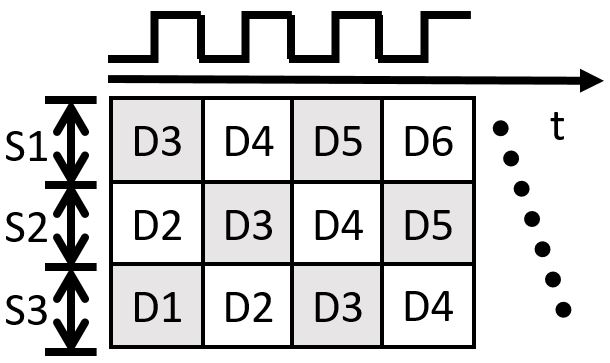
\includegraphics[width=.5\textwidth]{pipeline-w-data.jpg} \\
(a) \vspace{3pt} \\
{
\begin{lstlisting}[escapechar=@]
    r = read_input_port (in);
S1: y = mem[r.x]+1;
S2: mem[r.x] = y;
    set_output_port (out, y);
\end{lstlisting} 
}\\
(b) \vspace{3pt}\\
{
\small
\begin{lstlisting}[escapechar=@]
    r = read_input_port (in);
P1: if ( r.x == buf_addr ) {
       y_temp = buf_val;
    } else {
       y_temp = mem[r.x];
    }
    mem[buf_addr] = buf_val;   
S1: y = y_temp + 1;
S2: buf_addr = r.x;
    buf_val  = y;
    set_output_port (out, y);
\end{lstlisting} 
}\\
(c)
\end{tabular}
\caption{Examples of memory dependency. (a) No dependency. S$n$ represents a stage of the pipeline, D$n$ is a data. (b) Memory dependency occurs when state is stored in memory and needs to be updated. (c) Solving memory dependency using delayed write.}

\label{clicknp:fig:dependency}
\end{figure}

% registers
\egg{
\smalltitle{Use registers.}
Unlike a CPU, which executes instructions in memory sequentially, an FPGA synthesizes 
operations into hardware logic and stores data in registers, thereby 
enabling parallel evaluation.
For instance, in Figure~\ref{clicknp:fig:dependency}(a), a CPU may require two cycles 
to execute \textbf{S1} and \textbf{S2}, whereas in an FPGA, the values of variables 
\textit{y} and \textit{z} can be evaluated in a single cycle using 
combinational logic, provided all variables are stored in registers.
FPGAs typically have a large number of registers, for example, 697Kbit for Altera 
Stratix V, and therefore \name\ aggressively assigns scalar variables 
to registers to enhance parallelism.
}

%\smalltitle{Remove pseudo-dependency.}
A subtle issue arises when using the \textbf{struct} data structure. 
Figure \ref{clicknp:fig:memscattering}(a) illustrates such an example, where a hash table is used to maintain the count for each stream. 
There will be a memory dependency between \textbf{S2} and \textbf{S1}, even though they are accessing different fields of the \textbf{struct}. 
The reason is that almost all current high-level synthesis tools treat the \textbf{struct} data structure as a single data with a larger bit width -- equal to the size of the \textbf{struct}, and use only one arbiter to control access. 
This type of memory dependency is termed \textit{pseudo-dependency}. 
Physically, the two fields \textit{key} and \textit{cnt} can be located at different memory locations. 
To address this issue, \name employs a technique called \textit{memory scattering}, which automatically converts the \textbf{struct} array into several independent arrays, each used to store a field in the \textbf{struct}. Each array is allocated different BRAM, so they can be accessed in parallel (Figure \ref{clicknp:fig:memscattering}(b)). 
After implementing \textit{memory scattering}, \textbf{S1} is no longer dependent on \textbf{S2}, thus eliminating the pseudo-dependency. 
In general, if all accesses to an array can be divided into several disjoint equivalence classes, with the access address range of each class not overlapping, \textit{memory scattering} can be applied, converting the address range accessed by each equivalence class into an independent array \footnote{For example, in the case of Figure \ref{clicknp:fig:memscattering}, S1 accesses addresses divisible by 16 remainder 0 ~ 7, S2 accesses addresses divisible by 16 remainder 8 ~ 15.}. 
It is worth noting that memory scattering is only applicable to components in FPGA, and is disabled if the component runs on the host CPU.

\subsubsection{Balancing Pipeline Stages}
Ideally, each stage in a processing pipeline should operate at the same speed, meaning it processes data in one clock cycle. However, if the processes of each stage are unbalanced and some stages require more clock cycles than others, these stages will limit the overall throughput of the pipeline. For instance, in Figure \ref {clicknp:fig:unbalance} (a), \textbf {S1} is a loop operation. Since each iteration requires one cycle (\textbf {S2}), the entire loop will take $N$ cycles to complete, significantly reducing the pipeline throughput. Figure \ref {clicknp:fig:unbalance} (b) presents another example, where a BRAM cache is implemented for the global table (\textit {gmem}) in DDR. Although the "else" branch rarely hits, it creates a fat stage in the pipeline (requiring hundreds of clock cycles). The high-level synthesis compiler we use reserves the worst-case number of clock cycles for each stage, so even if the fat stage is rarely used, it greatly affects the processing speed of the entire pipeline.

\begin{figure}
\lstset{style=numbers}

\lstset{ emph={%
 element, init, state, handler, signal,include,state\_machine, goto_state
}, emphstyle={\bfseries},
morekeywords={get_input_port,read_input_port,from_tor, to_tor, set_output_port, host, begin, VLAN, IPv4, GRE} 
}
\centering

\begin{tabular}{c}
{
\small
\begin{lstlisting}[escapechar=@]
.handler {
   r = read_input_port (in);
   ushort *p = (ushort*) &r.fd.data;
S1: for (i = 0; i<N; i++) {
S2:  sum += p[i];
   }
   set_output_port (out, sum);
}
\end{lstlisting} 
} \\
(a) \vspace{3pt} \\
{
\small 
\begin{lstlisting}[escapechar=@]
.handler {
   r = read_input_port (in);
   idx = hash (r.x);
S1: if ( cache[idx].key == r.x ) {
     o = cache[idx].val;
S2: } else {
     o = gmem[r.x];
     k = cache[idx].key;
     gmem[k] = cache[idx].val;
     cache[idx].key = r.x;
     cache[idx].val = o;
   }
   set_output_port (out, o);
}
\end{lstlisting} 
} \\
(b) \vspace{3pt} 
\end{tabular}

\caption{Unbalanced pipeline stages.}
\label{clicknp:fig:unbalance}

\end{figure}

\name employs two strategies to balance the stages within the pipeline. Firstly, it unrolls loops to the maximum extent possible. 
Loop unrolling can break down a loop into a series of minor operations that can be executed in parallel or in a pipeline.
It's important to note that unrolling a loop will duplicate the operations in the loop body, thereby increasing the area cost.
Hence, it may only be suitable for loops with simple loop bodies and a small number of iterations.
In network functions, such small loops are quite common, such as calculating checksums, shifting packet payloads, or iterating over various possible configurations.
The \name{} compiler provides an \textbf {unroll} directive to unroll loops.

While many high-level synthesis tools support unrolling loops with known iteration counts, many real-world applications have loops with variable iteration counts.
However, in network functions, the upper limit of the loop iteration count can often be determined, such as the maximum length of a packet.
Since the iterator of a loop is often used as an array index, in this case, the upper and lower bounds of the iterator can be determined based on the size of the array \footnote{\name{} does not support dynamic memory allocation, so the size of all arrays can be statically determined at compile time.}.
There are also some loops where the upper limit of the iterator is a constant or a simple expression composed of other loop iterators, in which case the maximum value of the upper limit expression can be calculated.
For cases where the compiler cannot automatically determine the loop iteration count and \texttt{while} loops without explicit iterators, \name allows programmers to specify the upper limit of the loop count through \texttt{pragma}.
Once the upper limit of the loop count is determined, \name wraps the loop body with an \texttt{if} statement representing the loop condition, replaces the \texttt{continue} and \texttt{break} statements in the loop body, and then duplicates it.

For the computation shown in Figure \ref {clicknp:fig:unbalance} (a), memory dependencies need to be resolved after loop unrolling, because the variable \texttt{sum} is written and read multiple times. After loop unrolling, \name expands scalar variables into \emph{static single assignment} form, so that each variable is assigned only once, which can eliminate this kind of memory dependency. Essentially, static single assignment and delayed writing both increase memory space to improve parallelism.

The second technique involves separating different types of operations within a single component if it has both fast and slow operations. For instance, in a cache component's implementation, as depicted in Figure \ref {clicknp:fig:unbalance} (b), the slower "else" branch is relocated to another component. This allows the fast path and slow path to operate asynchronously. If the cache miss rate is extremely low, the entire component's processing speed is determined by the fast path. As shown in Figure \ref{clicknp:fig:async}, the \name compiler offers an "\texttt{async}" primitive. Users can insert code blocks enclosed in \texttt{async \{ \}} in the \texttt{handler}. The code inside will be compiled into a new component and connected to the original component through a pipeline. The original component serializes and sends the variables used in the asynchronous component, then waits for the asynchronous component to complete. Once the asynchronous component is finished, it sends the written variables that the original component will continue to use back to the original component.

\begin{figure}[htbp]
	\small
	\lstset{ emph={%
			element, init, state, handler, signal,include,state\_machine, goto_state, async
		}, emphstyle={\bfseries},
		morekeywords={get_input_port,read_input_port,from_tor, to_tor, set_output_port, host, begin, VLAN, IPv4, GRE} 
	}
	\centering
	\begin{tabular}{c}
\begin{lstlisting}
.handler {
  r = read_input_port (in);
  idx = hash (r.x);
  if (cache[idx].key == r.x) {
    o = cache[idx].val;
  } else {
    k = cache[idx].key;
    v = cache[idx].val;
    .async {
      o = gmem[r.x];
      gmem[k] = v;
    }
    cache[idx].key = r.x;
    cache[idx].val = o;
  }
  set_output_port (out, o);
}
\end{lstlisting}
	\end{tabular}
	\caption{Example of Async primitive.}
	\label{clicknp:fig:async}
\end{figure}

\iffalse
\begin{figure}
	
	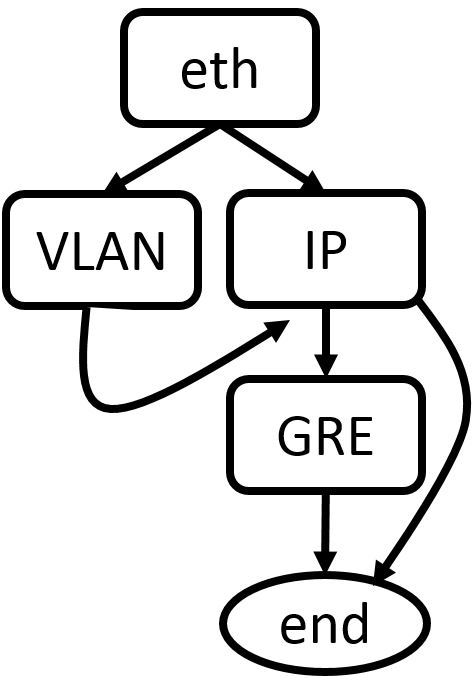
\includegraphics[width=.15\textwidth]{fsm1.jpg} \\
	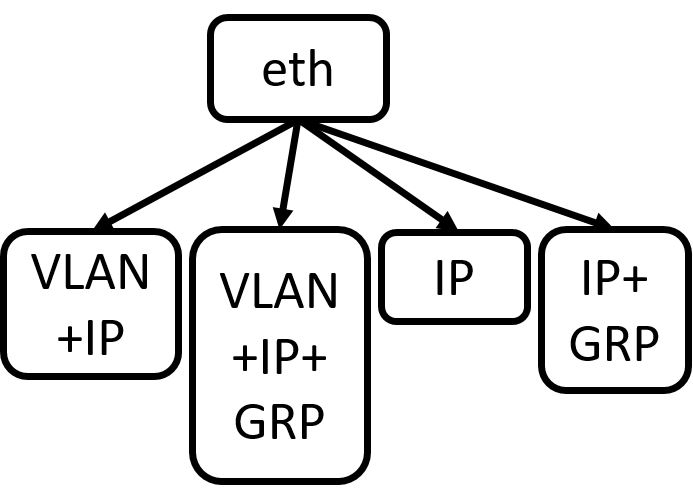
\includegraphics[width=.2\textwidth]{fsm2.jpg} \\
	
	\caption{FSM expansion. }
	\label{clicknp:fig:fsm-expansion}
\end{figure}

\smalltitle{Expand code.} \name\ provides several tools to assist programmers in expanding code, trading off FPGA area for speed.
One common code expansion is to unroll loops. Additionally, \name\ provides the \textit{.repeat} directive to expand code according to
a template.
Finally, \name\ can also aid in expanding a \textit{finite state machine} (FSM).
Figure~\ref{clicknp:fig:memscattering}(c) presents such an example in the packet header parser.
The \textbf{.state\_machine} directive serves two functions. Firstly, it offers programmers a declarative way to write an FSM by defining
states and their transitions (using \textbf{.goto\_state}).
Secondly, it also expands the FSM to achieve more parallelism. 
For instance, Figure~\ref{clicknp:fig:memscattering}(d) displays the parsing tree that is described according to the code piece in Figure~\ref{clicknp:fig:memscattering}(c).
However, the \name\ compiler can automatically expand the FSM to an equivalent, but significantly flattened FSM, as depicted in Figure~\ref{clicknp:fig:memscattering}(e). Now every header can be parsed in one cycle -- all parsing paths can be evaluated in parallel, 
instead of up to 4 cycles (Figure~\ref{clicknp:fig:memscattering}(d)).

\fi
